% !TEX root = Bachelorarbeit_Paul_Zilewitsch.tex
\section{Umsetzung}

\subsection{Erweiterung des bestehenden Service Desk Moduls}
\noindent
Grundlage für die Erweiterung ist die bereits erwähnte Microsoft Exchange Web Services Managed API 2.2, die kostenlos zum Download von Microsoft angeboten wird. Voraussetzung für diese API ist ein Betriebssystem von Windows (mindestens Windows 7) und das .NET Framwork 3.5 oder höher.\footnote{Website:\cite{DownloadAPI}}\newline 
Da diese API bereits in GEBman10 für das Versenden von E-Mails integriert wurde, konnte direkt ohne zusätzlichen Aufwand auf die Funktionalitäten zugegriffen werden. Wichtig war lediglich das Einfügen des Assemblerverweises in die entsprechenden Projektmappenordner. Um nicht den vollständigen Namespace jeder Klasse ausschreiben zu müssen, wurde außerdem die using-Direktive in den Klassen MailsToObjectsFactory und TicketHandler hinzugefügt.

\begin{figure}[h!]
\centering
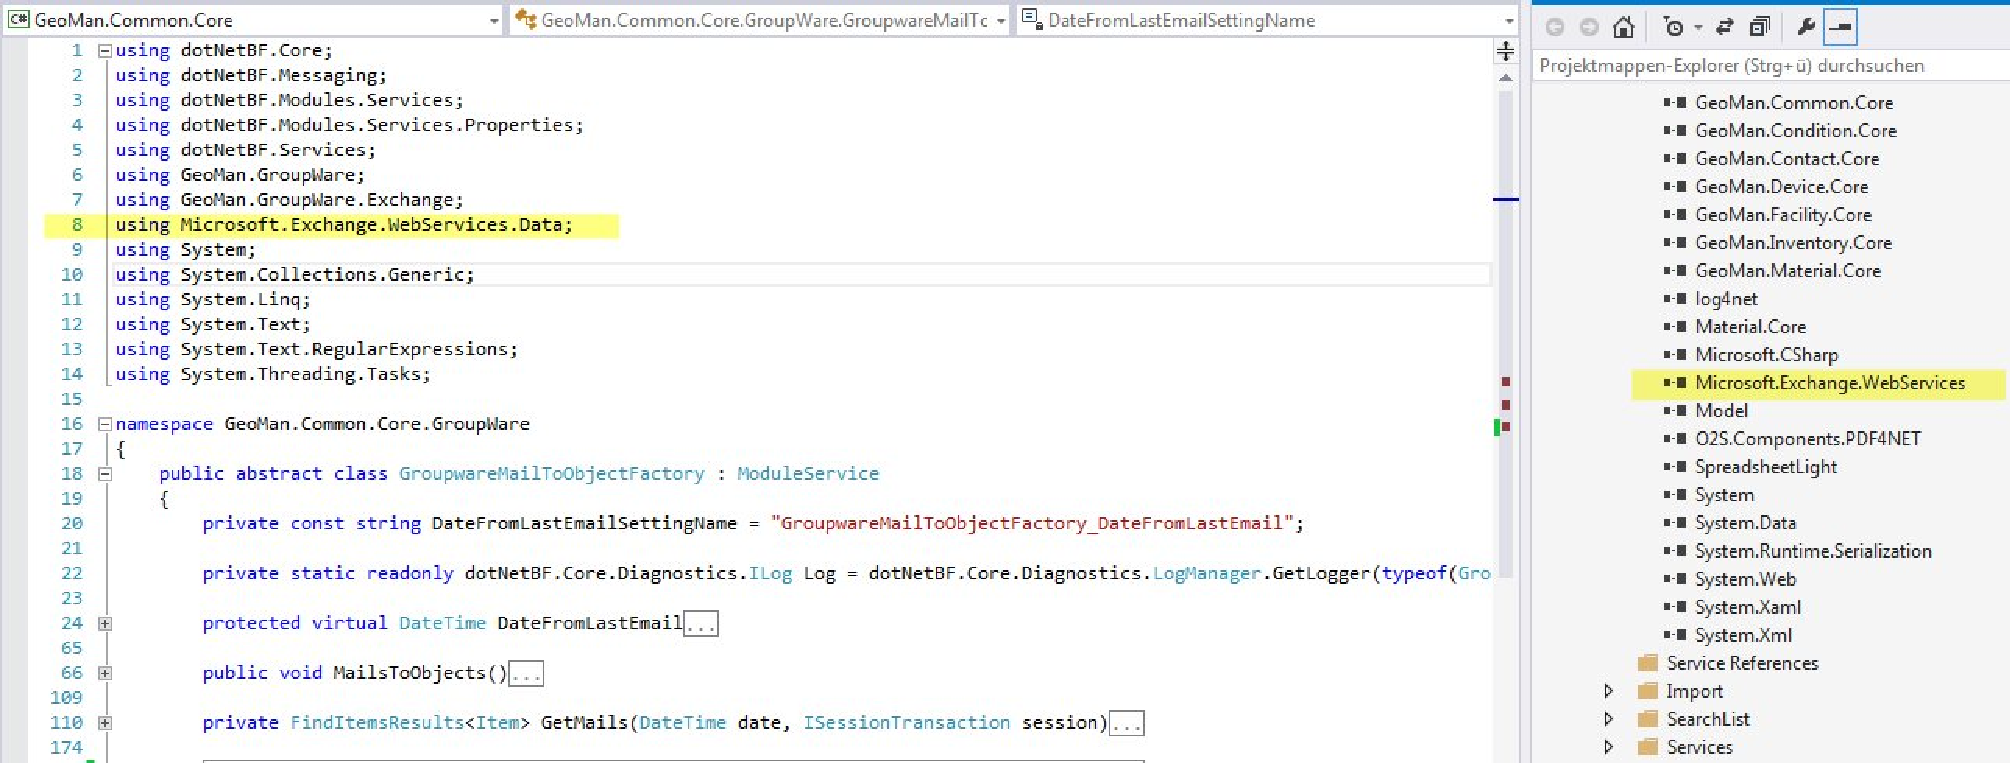
\includegraphics[width=0.75\textwidth]{Abbildungen/Screenshot_Verweise.pdf}
	\caption[Verweise]{Entwurfsmuster Fabrikmethode, Quelle: eigene Darstellung}
	\label{fig:Verweise}
\end{figure}

\noindent
Bei der Implementierung wurde sich stark an das Fabrikmethoden-Entwurfsmuster gehalten. Bevor hierauf näher eingegangen wird, sollte das Entwurfsmuster näher erläutert werden.\\
\noindent
Die Fabrikmethode (Factory Method) ist ein Erzeugungsmuster, bei dem die Objekterstellung von der Objektverarbeitung getrennt wird. Hierbei wird die Unterklasse durch eine abstrakte Methode der Oberklasse erzeugt.\footnote{Vgl. \citeauthor{PatternsKompakt} \citeyear{PatternsKompakt}, S.34ff.} Dieses Entwurfsmuster wurde auch bei der Implementierung in GEBman10 verwendet. 

\begin{figure}[h!]
\centering
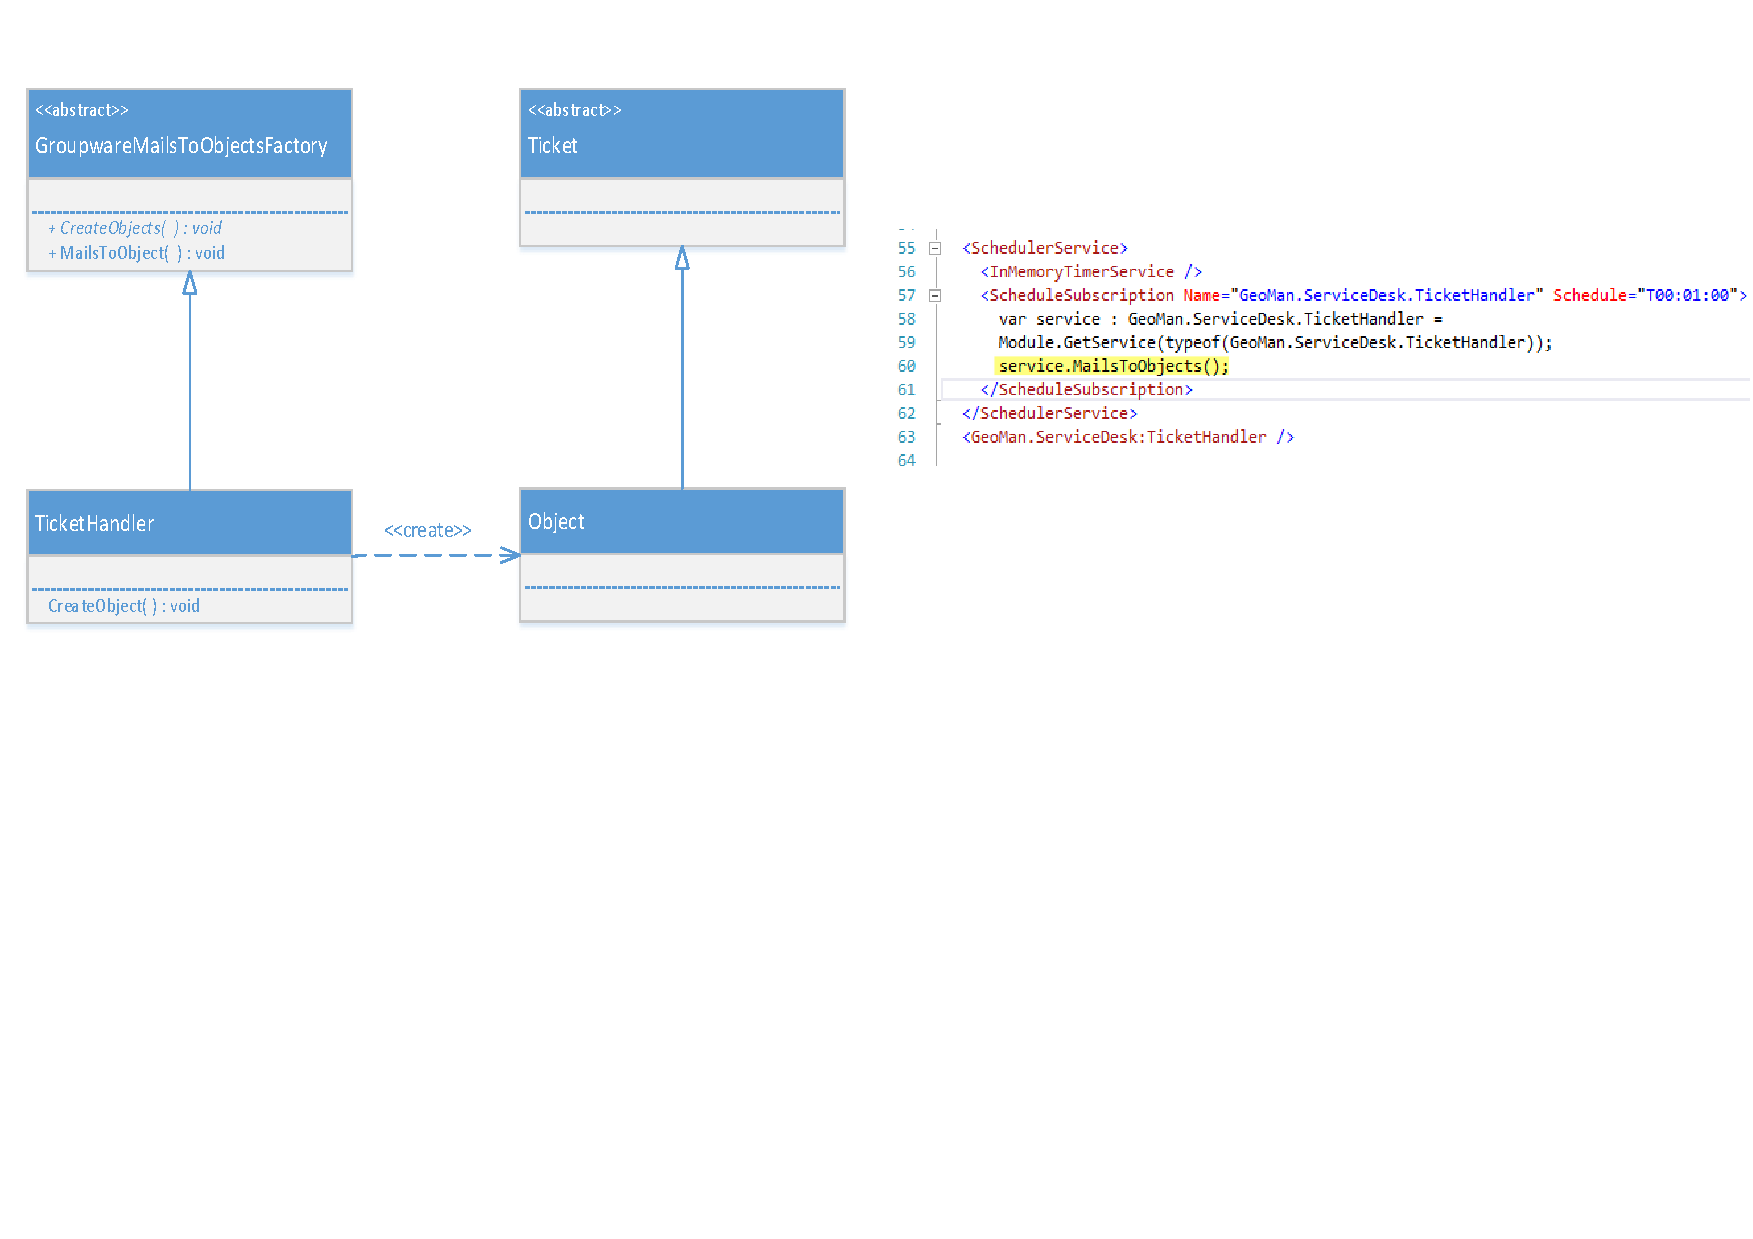
\includegraphics[width=0.75\textwidth]{Abbildungen/Entwurfsmuster.png}
	\caption[Entwurfsmuster Fabrikmethode]{Entwurfsmuster Fabrikmethode, Quelle: in Anlehnung an Eilebrecht, Starke (2013) S.35}
	\label{fig:Entwurfsmuster}
\end{figure}

\noindent
Bei jedem Intervall wird über den SchedulerService (Abbildung~\ref{fig:Entwurfsmuster} links) der Module Service TicketHandler instanziiert und die Methode MailsToObjects( ) der abstrakten Oberklasse aufgerufen. Die Fabrikmethode (rechts) macht deutlich, dass die abstrakte Klasse GroupwareMailToObjectFactory der Erzeuger und Ticket Handler der konkrete Erzeuger ist. Der konkrete Erzeuger wiederum erstellt dann ein Object über die abstrakte Methode CreateObject( ). Das Object ist in diesem Falle ein Ticket (Meldung). Vorteil dieses Entwurfsmusters ist die klare Kapselung des Erzeugers. Somit kann die Klasse GroupwareMailToObjectFactory auch für andere Module eingesetzt werden, die ebenfalls neue Objekte aus E-Mails erzeugen sollen. Eilebrecht und Starke sehen die Anwendung der Fabrikmethode als sinnvoll, wenn \enquote{eine Klasse die von ihr zu erzeugenden Objekte nicht im Voraus kennt}.\footnote{Vgl. \citeauthor{PatternsKompakt} \citeyear{PatternsKompakt}, S.34ff.} Genau dieser Anwendungsfall trifft hier zu und ist deshalb auch gerechtfertigt.\\






\subsection{Erläuterung der wichtigsten Klassen und Methoden}
\noindent
Wie erstellt man eine Meldung?
Testfälle?
Sicherheit?


\subsection{Fehlschläge/Erfahrungen}
\noindent
Bei der Implementierung in GEBman10 gab es zwei nicht vorhersehbare Probleme bei der Implementierung. Beide haben ihren Ursprung in der Managed API von Microsoft. In der Methode GetMails( ) werden alle Mails aus dem Posteingang des Exchange Servers abgefragt. Hierfür stellt die API eine Methode namens FindItems( ) zur Verfügung, die eine Collection aller Items liefert. Nun muss aber für diese Collection eine ItemView übergeben werden, die einen bestimmten Integerzahlenwert als festdefinierte Größe benötigt. Es ist also in der Theorie durchaus möglich, dass sich mehr Mails im Posteingang des Exchange Server befinden, als die Menge an Elementen der ItemView. Das hat zur Folge, dass alle Mails außerhalb der ItemView nicht in die Collection von der Methode FindItems( ) enthalten sind und auch nicht ausgewertet werden können. Um dieses Problem kurzer Hand zu beseitigen, wurde die ItemView Größe auf den maximalen Zahlenwert des Integerwertebereiches gesetzt. Dieses Wert zu überschreiten ist in der Praxis so gut wie unmöglich, der sich in einem 10-stelligen Bereich bewegt.\newline
%Es gäbe noch einen anderen WorkAround für dieses Problem, allerdings wäre diese Lösung mit mehr Aufwand verbunden. 
%https://msdn.microsoft.com/en-us/library/office/dd633698(v=exchg.80).aspx
Das zweite Problem bestand bei der Abfrage der neusten Mails vom Exchange Server, ebenfalls in der GetMails( )-Methode beschrieben. Bei jedem Abfrage Intervall wird der Zeitpunkt der zuletzt eingetroffenen Mail gespeichert. Beim nächsten Intervalldurchlauf werden dann nur alle Mails abgefragt, die ein aktuelles Datum besitzen. Hierfür bietet die Managed API einen SearchFilter an, der die Mails nach definierten Eigenschaften suchen kann. In diesem Fall ist war die Filter-Methode IsGreatherThan( ) optimal für dieses Vorhaben. Theoretisch hätten alle Mails abgefragt werden müssen, die ein \enquote{größeres} und damit aktuelleres Datum als die zuletzt eingetroffene Mail vom vorherigen Intervalldurchlauf hatten. Tatsächlich hat sich beim Debuggen gezeigt, dass der Filter zusätzlich ebenfalls die Mails liefert, die das gleiche Datum besitzen. Dadurch würde eine Mail in jedem Intervall zweimal gefiltert werden, was eine womöglich redundante Objekterzeugung zur Folge hätte. Wodurch dieses Problem entstand bleibt unklar. Umgangen wurde es, indem dem Datum der zuletzt eingetroffenen Mail nur eine Sekunde hinzugefügt wurde. Nach dieser minimalen Veränderung wurden die Mails korrekt gefiltert.

